% Chapter 2: User Documentation
\chapter{User Documentation}

\section{Introduction}

NutriFit is a comprehensive web-based Health and Fitness Management System designed to help users track their nutrition, manage workout routines, and monitor their health progress. The system provides an integrated platform where users can create personalized diet and workout plans, log their daily meals and exercises, set health goals, and visualize their progress through interactive charts and analytics.

The application is built using modern web technologies to ensure a responsive, fast, and user-friendly experience across different devices including desktops, tablets, and smartphones. Figure \ref{fig:framework} illustrates the overall framework and technology stack used in the NutriFit system.

\begin{figure}[H]
    \centering
    \includegraphics[width=0.9\textwidth]{images/framework-diagram.png}
    \caption{NutriFit System Framework and Technology Stack}
    \label{fig:framework}
\end{figure}

The framework diagram shown in Figure \ref{fig:framework} demonstrates the layered architecture of the system. At the presentation layer, the system uses Next.js 14 with React for building the user interface, styled with Tailwind CSS for responsive design. The application layer consists of Next.js API routes that handle business logic and data processing. The data layer utilizes Prisma ORM for database operations with SQLite as the database engine. Additional libraries such as Recharts for data visualization, JWT for authentication, and Bcrypt for password hashing complete the technology stack.

\section{System Requirements}

To run and use the NutriFit system, the following requirements must be met:

\subsection{Hardware Requirements}
\begin{itemize}
    \item \textbf{Processor:} Intel Core i3 or equivalent (minimum), Intel Core i5 or better (recommended)
    \item \textbf{RAM:} 4 GB (minimum), 8 GB or more (recommended)
    \item \textbf{Storage:} 500 MB free disk space for application and database
    \item \textbf{Display:} 1366x768 resolution (minimum), 1920x1080 or higher (recommended)
    \item \textbf{Network:} Internet connection for initial setup and updates
\end{itemize}

\subsection{Software Requirements}
\begin{itemize}
    \item \textbf{Operating System:} Windows 10/11, macOS 10.15+, or Linux (Ubuntu 20.04+)
    \item \textbf{Node.js:} Version 18.0 or higher
    \item \textbf{npm:} Version 9.0 or higher (comes with Node.js)
    \item \textbf{Web Browser:} Google Chrome 90+, Firefox 88+, Safari 14+, or Edge 90+
\end{itemize}

\subsection{User Requirements}
\begin{itemize}
    \item Basic computer literacy and web browsing skills
    \item Valid email address for account registration
    \item Understanding of basic health and fitness concepts
\end{itemize}

\section{Installation and Setup}

This section provides step-by-step instructions for installing and setting up the NutriFit system on a local machine.

\subsection{Installation Steps}

\textbf{Step 1: Install Node.js}

Download and install Node.js from the official website (https://nodejs.org). Verify the installation by opening a terminal or command prompt and running:

\begin{lstlisting}[language=bash, caption=Verify Node.js Installation]
node --version
npm --version
\end{lstlisting}

\textbf{Step 2: Clone or Download the Project}

Obtain the NutriFit project files either by cloning from a repository or extracting from a provided archive.

\textbf{Step 3: Install Dependencies}

Navigate to the project directory and install required packages:

\begin{lstlisting}[language=bash, caption=Install Project Dependencies]
cd nutrifit
npm install
\end{lstlisting}

\textbf{Step 4: Configure Environment Variables}

Create a \texttt{.env} file in the project root directory with the following configuration:

\begin{lstlisting}[caption=Environment Configuration]
DATABASE_URL="file:./prisma/dev.db"
JWT_SECRET="your-secret-key-here"
NODE_ENV="development"
\end{lstlisting}

\textbf{Step 5: Initialize Database}

Set up the database schema and seed initial data:

\begin{lstlisting}[language=bash, caption=Database Setup]
npx prisma generate
npx prisma migrate deploy
npx tsx prisma/seed.ts
\end{lstlisting}

\textbf{Step 6: Start the Development Server}

Launch the application:

\begin{lstlisting}[language=bash, caption=Start Application]
npm run dev
\end{lstlisting}

The application will be accessible at \texttt{http://localhost:3000}.

\section{User Interface Overview}

The NutriFit user interface is designed with simplicity and usability in mind. The system follows a consistent design pattern across all pages, featuring a clean layout, intuitive navigation, and responsive design that adapts to different screen sizes.

\subsection{Landing Page}

Figure \ref{fig:landing} shows the landing page, which serves as the entry point for new and returning users. The page features a hero section with the NutriFit branding, key features overview, and call-to-action buttons for registration and login.

\begin{figure}[H]
    \centering
    \includegraphics[width=0.9\textwidth]{images/landing-page.png}
    \caption{NutriFit Landing Page}
    \label{fig:landing}
\end{figure}

The landing page displayed in Figure \ref{fig:landing} presents a modern and welcoming interface with a gradient background featuring the NutriFit logo prominently at the top. The main heading "Transform Your Health Journey" immediately communicates the system's purpose. Below the heading, three key features are highlighted with icons: personalized nutrition plans, custom workout routines, and progress tracking. The page includes two prominent buttons for "Get Started" and "Sign In" to guide users toward registration or login.

\subsection{Dashboard}

After logging in, users are directed to the main dashboard shown in Figure \ref{fig:dashboard}. The dashboard provides an overview of the user's health status, recent activities, and quick access to all major features.

\begin{figure}[H]
    \centering
    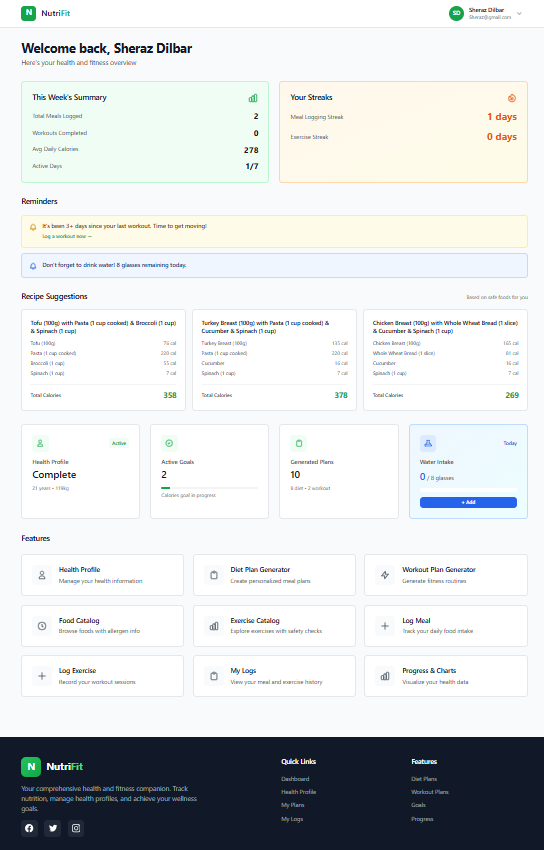
\includegraphics[width=0.9\textwidth]{images/dashboard.png}
    \caption{Main Dashboard Interface}
    \label{fig:dashboard}
\end{figure}

The dashboard interface in Figure \ref{fig:dashboard} features a navigation bar at the top with the NutriFit logo and user profile menu. The main content area displays summary cards showing today's calorie intake, workouts completed, water intake, and active goals. Below the summary cards, quick action buttons provide direct access to key features such as logging meals, logging exercises, generating diet plans, and creating workout plans. The dashboard also includes a recent activity section showing the user's latest logged meals and exercises.

\section{Functional Description}

This section describes each functional feature of the NutriFit system in detail, including screenshots and usage instructions.

\subsection{User Registration}

The registration feature allows new users to create an account in the system. Figure \ref{fig:register} shows the registration page interface.

\begin{figure}[H]
    \centering
    \includegraphics[width=0.8\textwidth]{images/register-page.png}
    \caption{User Registration Page}
    \label{fig:register}
\end{figure}

The registration page shown in Figure \ref{fig:register} features a split-screen design with branding information on the left and the registration form on the right. The form includes fields for full name, email address, password, and password confirmation. A notable feature is the password strength indicator that appears below the password field, displaying a visual representation of password strength using colored bars. The indicator shows "Weak," "Medium," or "Strong" based on password complexity, helping users create secure passwords. Real-time validation provides immediate feedback on input errors, such as invalid email format or password mismatch. Upon successful registration, users are automatically logged in and redirected to the dashboard.

\subsection{User Login}

The login feature provides secure access to existing user accounts. Figure \ref{fig:login} displays the login page interface.

\begin{figure}[H]
    \centering
    \includegraphics[width=0.8\textwidth]{images/login-page.png}
    \caption{User Login Page}
    \label{fig:login}
\end{figure}

The login page illustrated in Figure \ref{fig:login} maintains the same split-screen design as the registration page for consistency. The left side features motivational text and key benefits of using NutriFit, while the right side contains the login form with email and password fields. The form includes a "Remember Me" checkbox for convenience and a "Forgot Password" link for account recovery. Error messages are displayed prominently when login credentials are incorrect, and successful authentication redirects users to the dashboard with their session maintained using JWT tokens.

\subsection{Health Profile Management}

Users can create and manage their health profiles, which serve as the foundation for personalized recommendations. Figure \ref{fig:health-profile} shows the health profile creation interface.

\begin{figure}[H]
    \centering
    \includegraphics[width=0.9\textwidth]{images/health-profile.png}
    \caption{Health Profile Management Interface}
    \label{fig:health-profile}
\end{figure}

The health profile management interface in Figure \ref{fig:health-profile} provides a comprehensive form for users to input their personal health information. The form is organized into logical sections including basic information (age, gender, height, weight), activity level selection (sedentary, lightly active, moderately active, very active, extremely active), health goals (weight loss, weight gain, muscle gain, maintenance), and dietary restrictions. The allergen selection feature allows users to specify multiple allergens from a predefined list including milk, eggs, fish, shellfish, tree nuts, peanuts, wheat, soy, and gluten. The system uses this information to calculate BMI, determine caloric needs, and generate personalized diet and workout plans. The interface includes helpful tooltips and validation messages to guide users in providing accurate information.

\subsection{Diet Plan Generation}

The diet plan generation feature creates personalized meal plans based on user health profiles and preferences. Figure \ref{fig:diet-plan} illustrates the diet plan generation interface.

\begin{figure}[H]
    \centering
    \includegraphics[width=0.9\textwidth]{images/diet-plan-generation.png}
    \caption{Diet Plan Generation Interface}
    \label{fig:diet-plan}
\end{figure}

The diet plan generation interface shown in Figure \ref{fig:diet-plan} allows users to customize their meal plan parameters. Users can select the plan duration (7, 14, or 30 days), target daily calorie intake, number of meals per day (3, 4, or 5), and specific dietary goals. The system automatically suggests calorie targets based on the user's health profile but allows manual adjustment. Upon generation, the system creates a detailed meal plan that respects the user's allergen restrictions and dietary preferences. Each meal includes food items from the database with appropriate serving sizes to meet the calorie target. The generated plan is displayed in a structured format showing breakfast, lunch, dinner, and optional snacks with total calorie counts for each meal.

\subsection{Workout Plan Generation}

The workout plan generation feature creates customized exercise routines tailored to user fitness levels and goals. Figure \ref{fig:workout-plan} shows the workout plan generation interface.

\begin{figure}[H]
    \centering
    \includegraphics[width=0.9\textwidth]{images/workout-plan-generation.png}
    \caption{Workout Plan Generation Interface}
    \label{fig:workout-plan}
\end{figure}

The workout plan generation interface displayed in Figure \ref{fig:workout-plan} provides options for users to specify their workout preferences. Users can select the plan duration, workout intensity level (beginner, intermediate, advanced), focus area (full body, upper body, lower body, cardio, strength), and days per week for training. The system generates a structured workout plan that includes a variety of exercises from the database, organized by day and muscle group. Each exercise entry specifies the number of sets, repetitions, and estimated duration. The plan considers the user's fitness level to ensure appropriate exercise selection and intensity, preventing injury while promoting progress toward fitness goals.

\subsection{Meal Logging}

The meal logging feature allows users to record their daily food intake for tracking and analysis. Figure \ref{fig:meal-log} illustrates the meal logging interface.

\begin{figure}[H]
    \centering
    \includegraphics[width=0.9\textwidth]{images/meal-logging.png}
    \caption{Meal Logging Interface}
    \label{fig:meal-log}
\end{figure}

The meal logging interface shown in Figure \ref{fig:meal-log} provides an intuitive way to record meals throughout the day. Users can search for food items from the comprehensive food database, which includes nutritional information for each item. The search functionality supports partial matching and displays results in categorized groups (fruits, vegetables, proteins, grains, dairy, nuts, snacks). Users can select multiple food items, specify quantities, and assign them to meal types (breakfast, lunch, dinner, snack). The interface displays a running total of calories for the selected foods, helping users stay within their daily calorie targets. Each logged meal is timestamped and stored in the database for future reference and analysis.

\subsection{Exercise Logging}

The exercise logging feature enables users to track their workout activities and physical exercises. Figure \ref{fig:exercise-log} shows the exercise logging interface.

\begin{figure}[H]
    \centering
    \includegraphics[width=0.9\textwidth]{images/exercise-logging.png}
    \caption{Exercise Logging Interface}
    \label{fig:exercise-log}
\end{figure}

The exercise logging interface illustrated in Figure \ref{fig:exercise-log} allows users to record their workout sessions with detailed information. Users can search and select exercises from the database, which includes various types of activities such as cardio, strength training, flexibility exercises, and sports. For each exercise, users can specify the duration, number of sets and repetitions (for strength exercises), and intensity level. The interface calculates estimated calories burned based on the exercise type and duration. Users can log multiple exercises in a single session, and the system maintains a complete history of all workout activities for progress tracking and analysis.

\subsection{Progress Tracking and Analytics}

The progress tracking feature provides visual analytics of user health data over time. Figure \ref{fig:progress} displays the progress analytics interface.

\begin{figure}[H]
    \centering
    \includegraphics[width=0.9\textwidth]{images/progress-analytics.png}
    \caption{Progress Tracking and Analytics Interface}
    \label{fig:progress}
\end{figure}

The progress analytics interface shown in Figure \ref{fig:progress} presents comprehensive visualizations of user health data. The page includes summary statistics cards displaying total meals logged, workouts completed, average daily calories, and days tracked. Interactive charts show daily calorie intake trends using a line chart, daily workout frequency using a bar chart, and food category distribution using a pie chart. Users can select different time ranges (7 days or 30 days) to view their progress over various periods. The interface also includes a key insights section that provides personalized feedback based on the user's activity patterns. All charts are interactive, allowing users to hover over data points for detailed information. The page includes export functionality to download progress data in CSV format and print functionality to generate physical reports.

\subsection{Goal Management}

The goal management feature allows users to set, track, and manage their health and fitness goals. Figure \ref{fig:goals} shows the goal management interface.

\begin{figure}[H]
    \centering
    \includegraphics[width=0.9\textwidth]{images/goal-management.png}
    \caption{Goal Management Interface}
    \label{fig:goals}
\end{figure}

The goal management interface displayed in Figure \ref{fig:goals} enables users to create specific, measurable health goals. Users can set goals for weight targets, daily calorie intake, weekly workout frequency, water intake, or custom objectives. Each goal includes a title, description, target value, current progress, and deadline. The interface displays goals in organized cards showing progress bars and completion percentages. Users can mark goals as completed, edit existing goals, or delete goals that are no longer relevant. The system tracks goal progress automatically based on logged meals, exercises, and other activities, providing real-time updates on achievement status.

\subsection{Water Intake Tracking}

The water intake tracking feature helps users monitor their daily hydration levels. Figure \ref{fig:water} illustrates the water intake tracking interface.

\begin{figure}[H]
    \centering
    \includegraphics[width=0.8\textwidth]{images/water-intake.png}
    \caption{Water Intake Tracking Interface}
    \label{fig:water}
\end{figure}

The water intake tracking interface shown in Figure \ref{fig:water} provides a simple and effective way to log daily water consumption. Users can quickly add water intake in standard serving sizes (250ml glasses) with a single click. The interface displays a visual progress indicator showing the percentage of daily water goal achieved, along with the total amount consumed in milliliters. The recommended daily water intake is calculated based on the user's weight and activity level. Users can view their water intake history and trends over time to ensure consistent hydration habits.

\subsection{My Plans}

The My Plans feature provides access to all generated diet and workout plans. Figure \ref{fig:my-plans} shows the My Plans interface.

\begin{figure}[H]
    \centering
    \includegraphics[width=0.9\textwidth]{images/my-plans.png}
    \caption{My Plans Interface}
    \label{fig:my-plans}
\end{figure}

The My Plans interface illustrated in Figure \ref{fig:my-plans} displays all previously generated diet and workout plans in an organized grid layout. Each plan card shows key information including creation date, plan duration, calorie target (for diet plans) or intensity level (for workout plans), and summary statistics. Users can switch between diet plans and workout plans using tab navigation. The interface provides action buttons to view detailed plan information in a modal popup, print plans for offline reference, and delete plans that are no longer needed. The view details modal displays the complete plan with all meals or exercises organized by day, making it easy to follow the plan throughout its duration.

\subsection{My Logs}

The My Logs feature provides a comprehensive view of all logged meals and exercises. Figure \ref{fig:my-logs} shows the My Logs interface.

\begin{figure}[H]
    \centering
    \includegraphics[width=0.9\textwidth]{images/my-logs.png}
    \caption{My Logs Interface}
    \label{fig:my-logs}
\end{figure}

The My Logs interface displayed in Figure \ref{fig:my-logs} presents a chronological history of all user activities including meal logs and exercise logs. The interface uses tab navigation to switch between meal logs and exercise logs. Each log entry displays the date, time, items logged (foods or exercises), quantities, and total calories. Users can filter logs by date range to view specific periods. The interface includes action buttons to edit or delete log entries, allowing users to correct mistakes or remove accidental entries. Summary statistics at the top show total logs, average daily calories, and other relevant metrics for the selected time period.

\subsection{Food and Exercise Catalogs}

The system includes comprehensive catalogs of food items and exercises. Figures \ref{fig:food-catalog} and \ref{fig:exercise-catalog} show these catalog interfaces.

\begin{figure}[H]
    \centering
    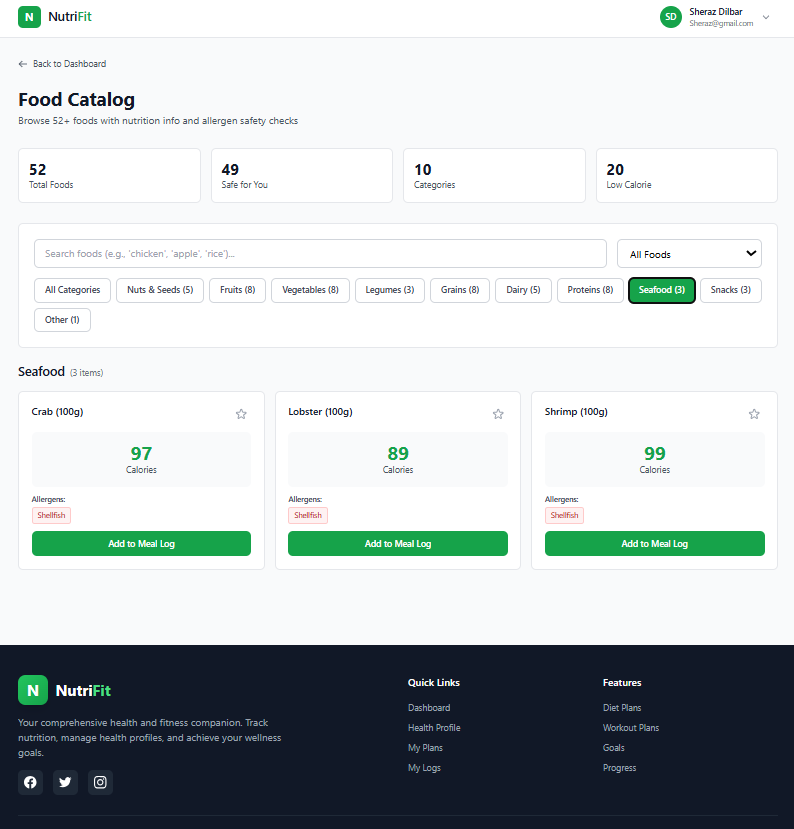
\includegraphics[width=0.9\textwidth]{images/food-catalog.png}
    \caption{Food Catalog Interface}
    \label{fig:food-catalog}
\end{figure}

The food catalog interface shown in Figure \ref{fig:food-catalog} displays all available food items organized by category. Each food item card shows the name, calorie content per serving, and allergen information. Users can search for specific foods using the search bar, filter by category, and mark foods as favorites for quick access during meal logging. The catalog includes 52 food items covering fruits, vegetables, proteins, grains, dairy products, nuts, and snacks, providing a comprehensive database for meal planning and logging.

\begin{figure}[H]
    \centering
    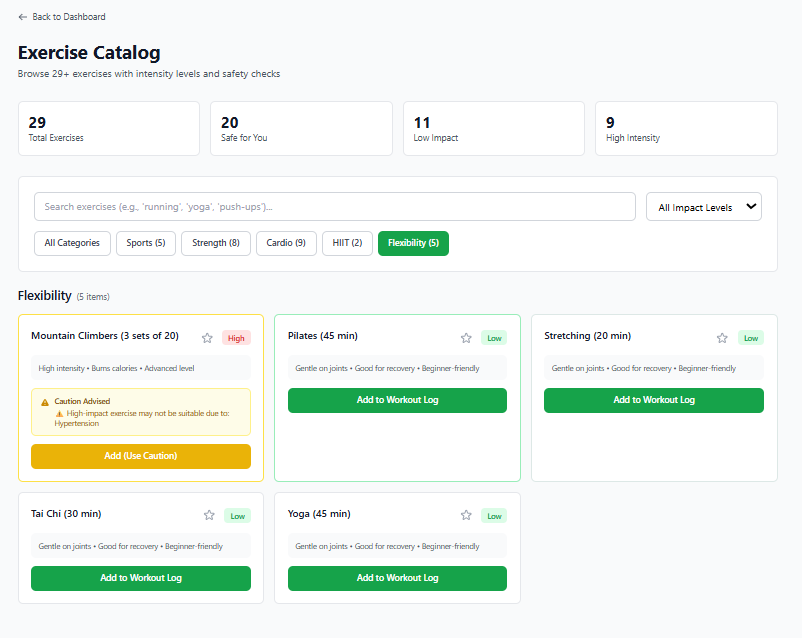
\includegraphics[width=0.9\textwidth]{images/exercise-catalog.png}
    \caption{Exercise Catalog Interface}
    \label{fig:exercise-catalog}
\end{figure}

The exercise catalog interface illustrated in Figure \ref{fig:exercise-catalog} presents all available exercises organized by type and impact level. Each exercise card displays the name, type (cardio, strength, flexibility, sports), and impact level (low, medium, high). Users can search for exercises, filter by type or impact level, and mark exercises as favorites. The catalog includes 29 exercises covering various fitness activities, ensuring users have diverse options for their workout routines.

\subsection{Settings and Profile Management}

The settings feature allows users to manage their account and preferences. Figure \ref{fig:settings} shows the settings interface.

\begin{figure}[H]
    \centering
    \includegraphics[width=0.9\textwidth]{images/settings.png}
    \caption{Settings and Profile Management Interface}
    \label{fig:settings}
\end{figure}

The settings interface displayed in Figure \ref{fig:settings} provides options for users to update their profile information, change password, and manage account settings. The interface is organized into sections including profile information (name, email), security settings (password change), and account management (delete account option). Users can update their health profile information, which automatically recalculates personalized recommendations. The password change feature includes current password verification and password strength validation for the new password. The account deletion option includes a confirmation dialog to prevent accidental data loss.

\section{Error Handling and Notifications}

The NutriFit system implements comprehensive error handling and user notification mechanisms to ensure a smooth user experience. Figure \ref{fig:notifications} shows examples of system notifications.

\begin{figure}[H]
    \centering
    \includegraphics[width=0.7\textwidth]{images/notifications.png}
    \caption{System Notifications and Error Messages}
    \label{fig:notifications}
\end{figure}

The notification system shown in Figure \ref{fig:notifications} displays toast messages for various user actions and system events. Success notifications appear in green with a checkmark icon, confirming successful operations such as meal logging, plan generation, or profile updates. Error notifications appear in red with an error icon, alerting users to issues such as invalid input, authentication failures, or server errors. Warning notifications appear in yellow, providing cautionary information such as duplicate meal logging or approaching calorie limits. Information notifications appear in blue, offering helpful tips or system updates. All notifications automatically dismiss after three seconds but can be manually closed by clicking the close button. The notification system ensures users receive immediate feedback on their actions, improving the overall user experience and reducing confusion.
